\subsection{Modulo Network}
	\label{sec:network}
	
	El módulo \textit{Network} (ver Figura \ref{fig:GeneralSystem}) es el encargado de instanciar todos los elementos ferroviarios presentes en la red de grafos generada por el RNA e interconectarlos como el RNA indica. Es el módulo que mas recursos de la FPGA utiliza y donde más se hace énfasis en el uso óptimo de los recursos. Para lograr esto, se prioriza la máxima descentralización posible de los módulos instanciados internamente, de forma tal que cada uno de ellos solo dependa de la mínima cantidad necesaria de módulos, evitando conexiones innecesarias. El diagrama de bloques de la máquina de estados finitos con camino de datos diseñado para lograr este objetivo se muestra en la Figura \ref{fig:Network_module}.
	
	\begin{figure}[H]
		\centering
		\includegraphics[width=1\textwidth]{Figuras/Network_module.png}
		\centering\caption{FSMD del módulo \textit{Network}.}
		\label{fig:Network_module}
	\end{figure}
	
	Los módulos de \textit{NetElements}, \textit{Routes} y \textit{Signals} son obligatorios ya que se encuentran presentes en la mínima red ferroviaria aceptada por el RNA. En cambio, los módulos de \textit{SingleSwitches}, \textit{DoubleSwitches}, \textit{ScissorCrossings} y \textit{LevelCrossings} son opcionales y dependen de que existan en la locación. Es decir, si un elemento ferroviario no existe, no solamente no serán instanciado por el ACG, sino que tampoco se generarán archivos que definan sus módulos, señales auxiliares que los interconecten a otros módulos ni tampoco entradas o salidas en otros módulos, destinados a este elemento. De esta manera, se reduce la complejidad del sistema enormemente al implementar solamente los puertos, señales, módulos y conexiones que serán utilizados por el sistema de enclavamiento.
	
	Para garantizar la descentralización de la red, a todos los elementos ferroviarios con entidad física, es decir, todos los mencionados (vías, pasos a nivel, cambios de vías, señales), excepto las rutas que son entidades abstractas, se les implementa la propiedad de enclavamiento. El enclavamiento de un elemento puede presentar tres estados, tal como se describe en la Tabla \ref{Tab:interlock_states}.
	
		\begin{table}[!h]
		{
			\caption{Estados de enclavamiento de cada elemento ferroviario.}
			\label{Tab:interlock_states}
			\centering
			\resizebox{1\textwidth}{!}{
			\begin{tabular}{ p{5cm} p{4cm} p{4cm} }
				\hline	
				Liberado & Reservado & Enclavado \\	
				\hline
				Solicitado por al menos una ruta u opera de forma automática.& 
				Operado solamente por la ruta que lo reservó.&
				Depende de sí mismo y de la ruta que lo enclavó.\\
				\hline
			\end{tabular}
			}
		}
		\end{table}
	
	Todo elemento se encuentra por defecto en el estado liberado y puede ser solicitado por cualquier ruta. Tan pronto una ruta envía el comando de reserva al elemento, pasa a estar en estado reservado y ninguna otra ruta podrá hacer uso de este elemento. Finalmente, si la ruta ha podido reservar todos los elementos necesarios para cumplir las condiciones para ser habilitada, enviará la señal de enclavamiento a todos los elementos involucrados, lo que evita que puedan ser comandados por otras rutas. Esto incluye tanto a la ocupación de vías (\textit{NetElements}) como a las señales (\textit{Signals}), pasando por todos los cambios de vías (\textit{SingleSwitches}, \textit{DoubleSwitches} y \textit{ScissorCrossings}) y barreras de pasos a nivel (\textit{LevelCrossings}). De esta manera el ACG se asegura que cada elemento sea controlado por una única ruta por vez o de forma automática si ninguna ruta demanda su uso.
	
	Para generalizar y modelizar el comportamiento dinámico de los elementos ferroviarios se utilizaron redes de Petri \cite{Paper_64,Paper_65,Paper_88,Paper_94,Paper_95,Paper_123,Paper_196}. Una red de Petri es la representación gráfica de un modelo matemático de autómatas concurrente. Las mismas están formadas por lugares (los estados), las transiciones que indican las condiciones para pasar de un lugar a otro, y los arcos que conectan lugares y transiciones. Las redes de Petri puede poseer uno o mas tokens que representan en que estado se encuentra el sistema. Algunas redes de Petri admiten mas de un token por red, o incluso mas de un token por lugar. En el caso del sistema de enclavamiento se definieron solamente redes de Petri con un único token por red, siendo que el sistema solo puede adoptar un estado en cada momento. En la Figura \ref{fig:Interlocking_petri} se visualiza el modelo matemático del enclavamiento de un elemento ferroviario genérico.
	
	\begin{figure}[H]
		\centering
		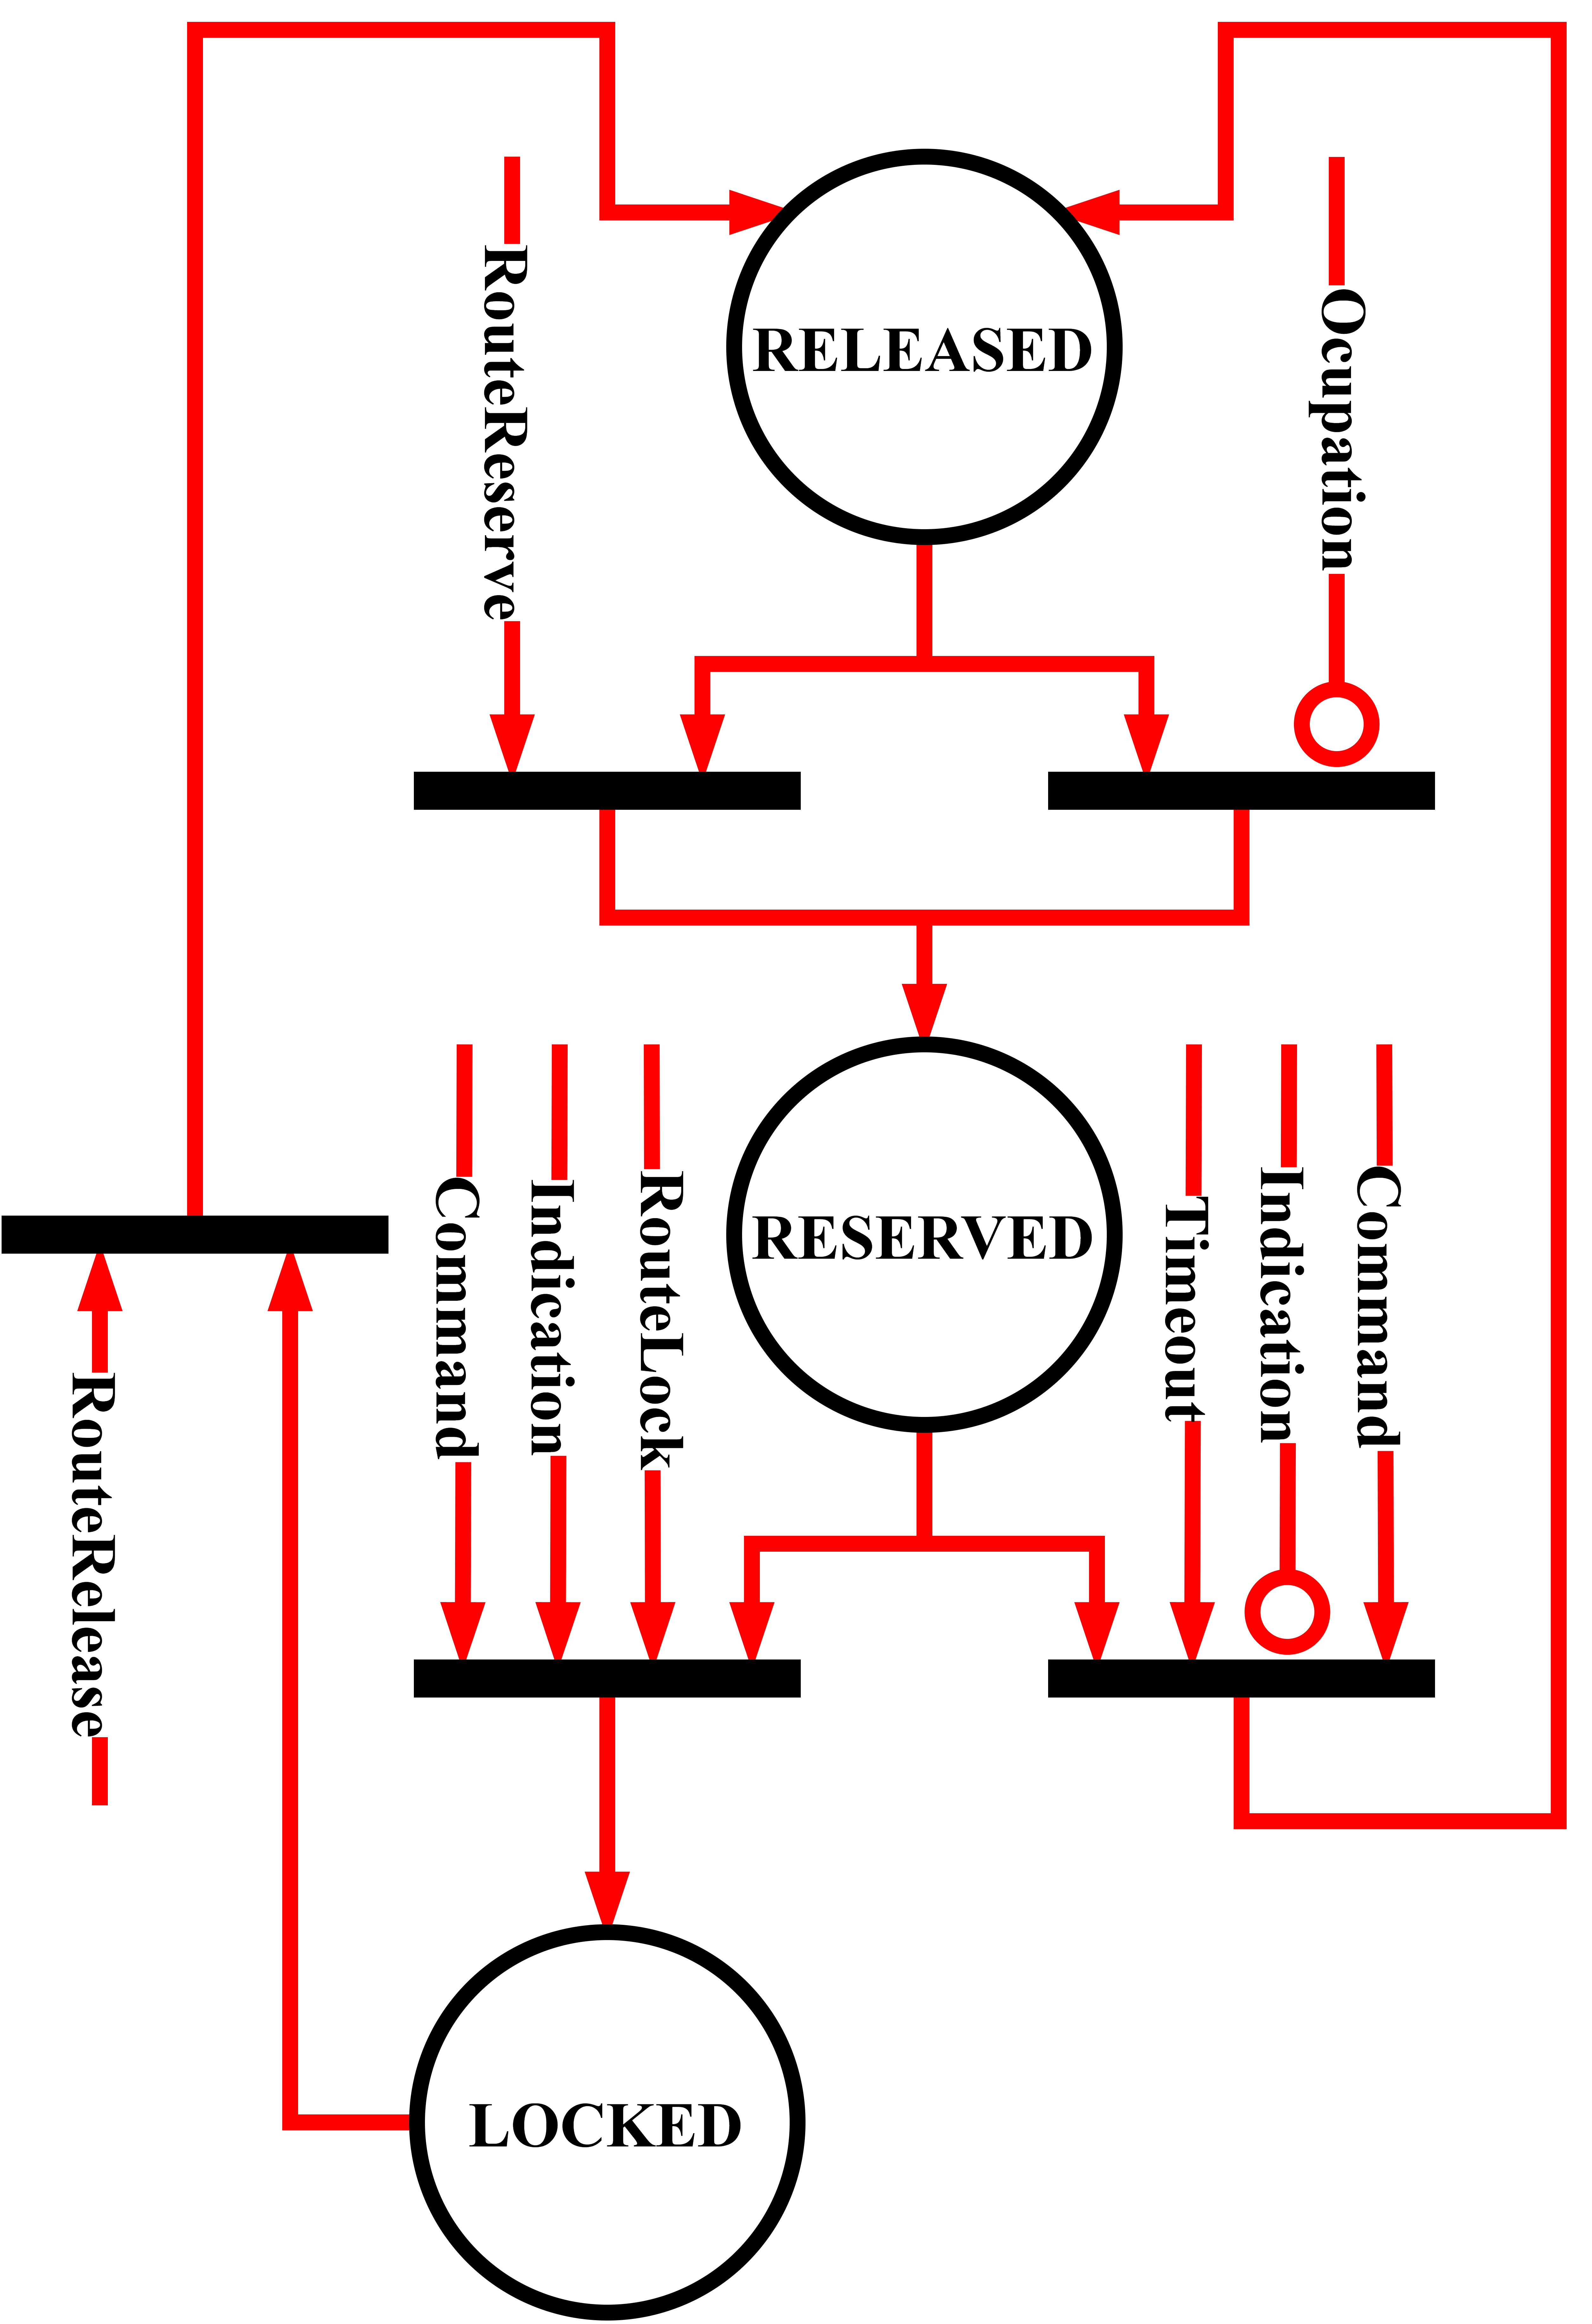
\includegraphics[width=0.7\textwidth]{Figuras/INT_petri}
		\centering\caption{Red de Petri del modelo dinámico de enclavamiento de elementos ferroviarios genéricos.}
		\label{fig:Interlocking_petri}
	\end{figure}
	
	En la Figura \ref{fig:Interlocking_petri} se oberva que la transición de un elemento ferroviario del estado liberado a reservado no solo puede darse por el pedido expreso de una ruta que lo solicite, sino también de facto al ocuparse los netElements cercanos al elemento, lo cual inicia lo que se denomina 'bloqueo por ocupación' (ver Sección \ref{sec:function_1}). Esto protege al sistema al impedir que otras rutas soliciten un cambio de estado de un elemento que esta siendo usado por una formación que no ha solicitado ningún permiso, lo que reduce el riesgo de accidentes por descarrilamiento o colisión. 
	
	La red de Petri también deja explícito la inclusión de un timeout para las reservas, con un valor por defecto de 7 segundos, configurable por el usuario. De no cumplirse que el comando y la indicación coincidan dentro del tiempo estipulado, el elemento es liberado, siempre que no se encuentren formaciones cercanas. Las transición de reserva a enclavamiento requiere que tanto el comando como la indicación coincidan y que la ruta solicite el enclavamiento al haber confirmado que todas las condiciones de ruta se han cumplido y es inminente su habilitación. El elemento ferroviario deja de estar enclavado cuando la ruta lo solicita expresamente, momento en el cuál pasa a estar liberado para que otras rutas puedan usarlo.
	
	A diferencia de los módulos explicados en secciones anteriores, donde cada módulo era instanciado una vez, los módulos que modelan elementos ferroviarios, con entidad física (cómo un cambio de vías simple) o abstracta (cómo una ruta ferroviaria), son instanciados tantas veces como unidades de éstos existan. Es por eso que, en las siguientes secciones, hablaremos de módulos genéricos a la hora de describir cada módulo. Estos módulos genéricos presentarán todas las entradas, salidas y funcionalidades que pueden tener, en caso de ser necesarias para la implementación del sistema de enclavamientos. Es trabajo del ACG determinar cuales de ellas deben ser implementadas y cuales no. Por ejemplo, si una ruta A requiere que una barrera X se encuentre baja, pero no tiene requerimientos respecto a las posiciones de los cambios porque la ruta A no los utiliza, entonces el ACG instanciará el módulo de la ruta A considerando en las entradas y salidas los estados de la barrera X y los comandos para operarla, interconectando el módulo de ruta A con el módulo de la barrera ferroviaria X. En cambio, el ACG no implementará ningún puerto destinado a los cambios de vías ni lo considerará en las funcionalidades del módulo de ruta A. De igual manera, el ACG conectará los estados de ocupación de vías correspondientes solamente a los módulos de los elementos ferroviarios que los necesitan y no la totalidad del vector de datos.
	
	\subsection{Módulo genérico de las barreras ferroviarias}

El módulo \textit{LevelCrossing} es el encargado de implementar el funcionamiento de las barreras ferroviarias en los pasos a nivel. El ACG utiliza la información otorgada por el RNA para determinar cuál es el netElement donde se sitúa el paso a nivel y cuales son los netElements mas próximos, para que puedan reportar su estado al módulo \textit{LevelCrossing}. Además, el ACG implementará todas las conexiones para cada una de las rutas en las cuales el paso a nivel sea condición necesaria para su habilitación. El diagrama de bloques de las máquinas de estado finitas con camino de datos diseñado para lograr este objetivo se muestra en la Figura \ref{fig:Network_module}.

\begin{figure}[H]
	\centering
	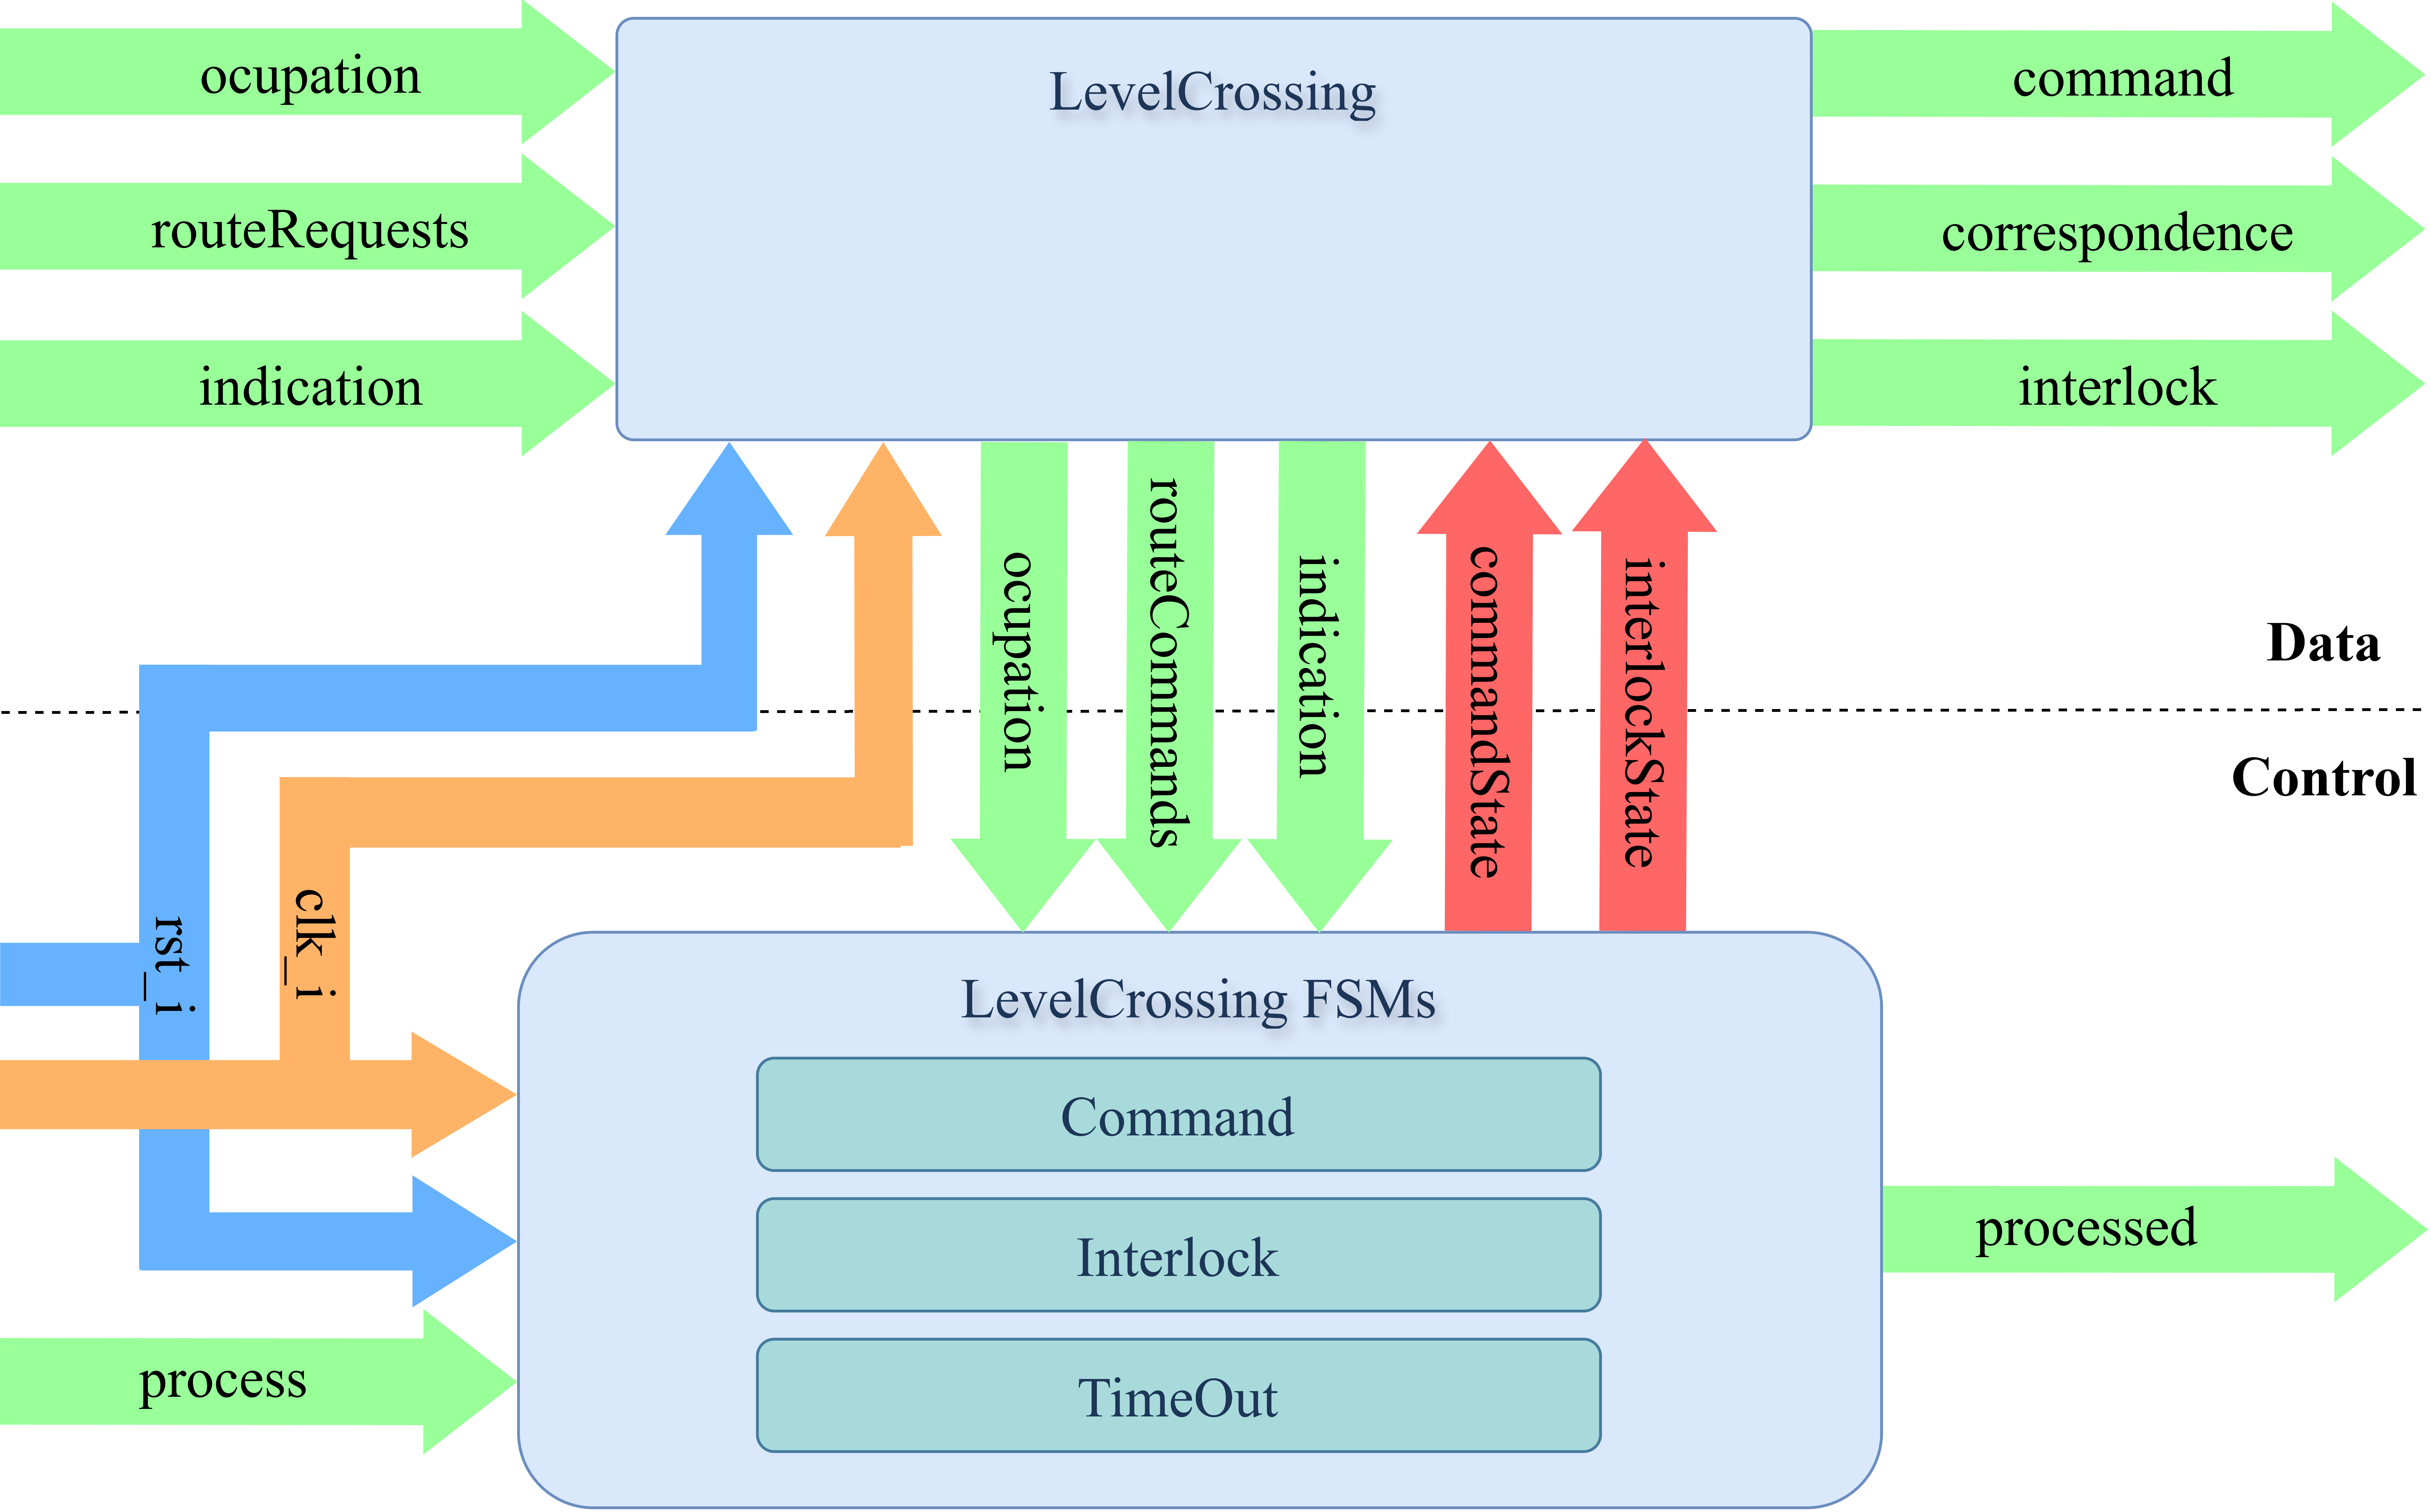
\includegraphics[width=1\textwidth]{Figuras/LCB_module}
	\centering\caption{FSMD del módulo genérico de \textit{LevelCrossing}.}
	\label{fig:LCB_module}
\end{figure}

Tal como se explicó en la Sección \ref{sec:switches}, las barreras ferroviarias también poseen comando, indicación y correspondencia. Comando para controlar la barrera, indicación para reportar su estado actual al módulo \textit{LevelCrossing} y correspondencia para declarar su estado final a la ruta que lo solicite. Además, el ACG implementará todas las conexiones necesarias a todas las rutas que tengan a la barrera en cuestión como condición necesaria de habilitación. Finalmente, el módulo \textit{LevelCrossing} tiene una salida que define su estado de enclavamiento frente a otras rutas que lo requieran.

El comportamiento de una barrera de paso a nivel genérico se define en la red de Petri de la Figura \ref{fig:LCB_Petri}. Una barrera se mantendrá en estado alto a menos que una ruta solicite que el brazo de barrera descienda o si los \textit{netElements} cercanos se encuentran ocupados. Durante la transición se espera la confirmación de que la barrera ha descendido mientras se mantiene la ocupación para terminar el movimiento en el estado bajo. Estado en el cual solo podrá salir si la ocupación termina y ninguna ruta solicita que la barrera se mantenga baja.

\begin{figure}[H]
	\centering
	\includegraphics[width=1\textwidth]{Figuras/LCB_petri}
	\centering\caption{Red de Petri del modelo dinámico de \textit{LevelCrossing}.}
	\label{fig:LCB_Petri}
\end{figure}

Durante el estado de transición la barrera tendrá 7 segundos para llegar al estado bajo. Al cumplirse el tiempo, si la indicación y el comando no coinciden y los textit{netElements} cercanos se encuentran libres, la barrera volverá al estado alto. Esto impide que el sistema habilite rutas cuando los actuadores de algún elemento se atascan o su indicación es diferente al comando que se ha enviado. La confirmación de la indicación otorga un grado de seguridad mayor al no asumir que un comando enviado implica automáticamente que al actuador se le impone dicho estado.
	\subsection{Módulo genérico de los cambios de vías simples}
	\label{sec:ACG_ssw}
	
	El módulo \textit{SingleSwitches} (ver Figura \ref{fig:GeneralSystem}) es el encargado de implementar el funcionamiento de los cambios de vías simples en la red ferroviaria. El ACG utiliza la información otorgada por el RNA para determinar cuales son los \textit{netElements} conectados mediante el cambio de vías, los \textit{netElements} más próximos. Esta información se utiliza para implementar las entradas del módulo \textit{SingleSwitches} donde se reporta el estado de ocupación de los \textit{netElements} (\textit{ocupation}). Además, se implementan las conexiones de indicación, comando y correspondencia para poder leer, escribir y reportar el estado del cambio de vías, respectivamente. Finalmente, el ACG implementa las conexiones a todas las rutas que buscarán controlar el cambio de vías y todo los mecanismos para obedecer solo a una de ellas, de cumplirse las condiciones. El diagrama de bloques de las máquinas de estado finitas con camino de datos diseñado para lograr este objetivo se muestra en la Figura \ref{fig:SSW_module}.
	
	\begin{figure}[H]
		\centering
		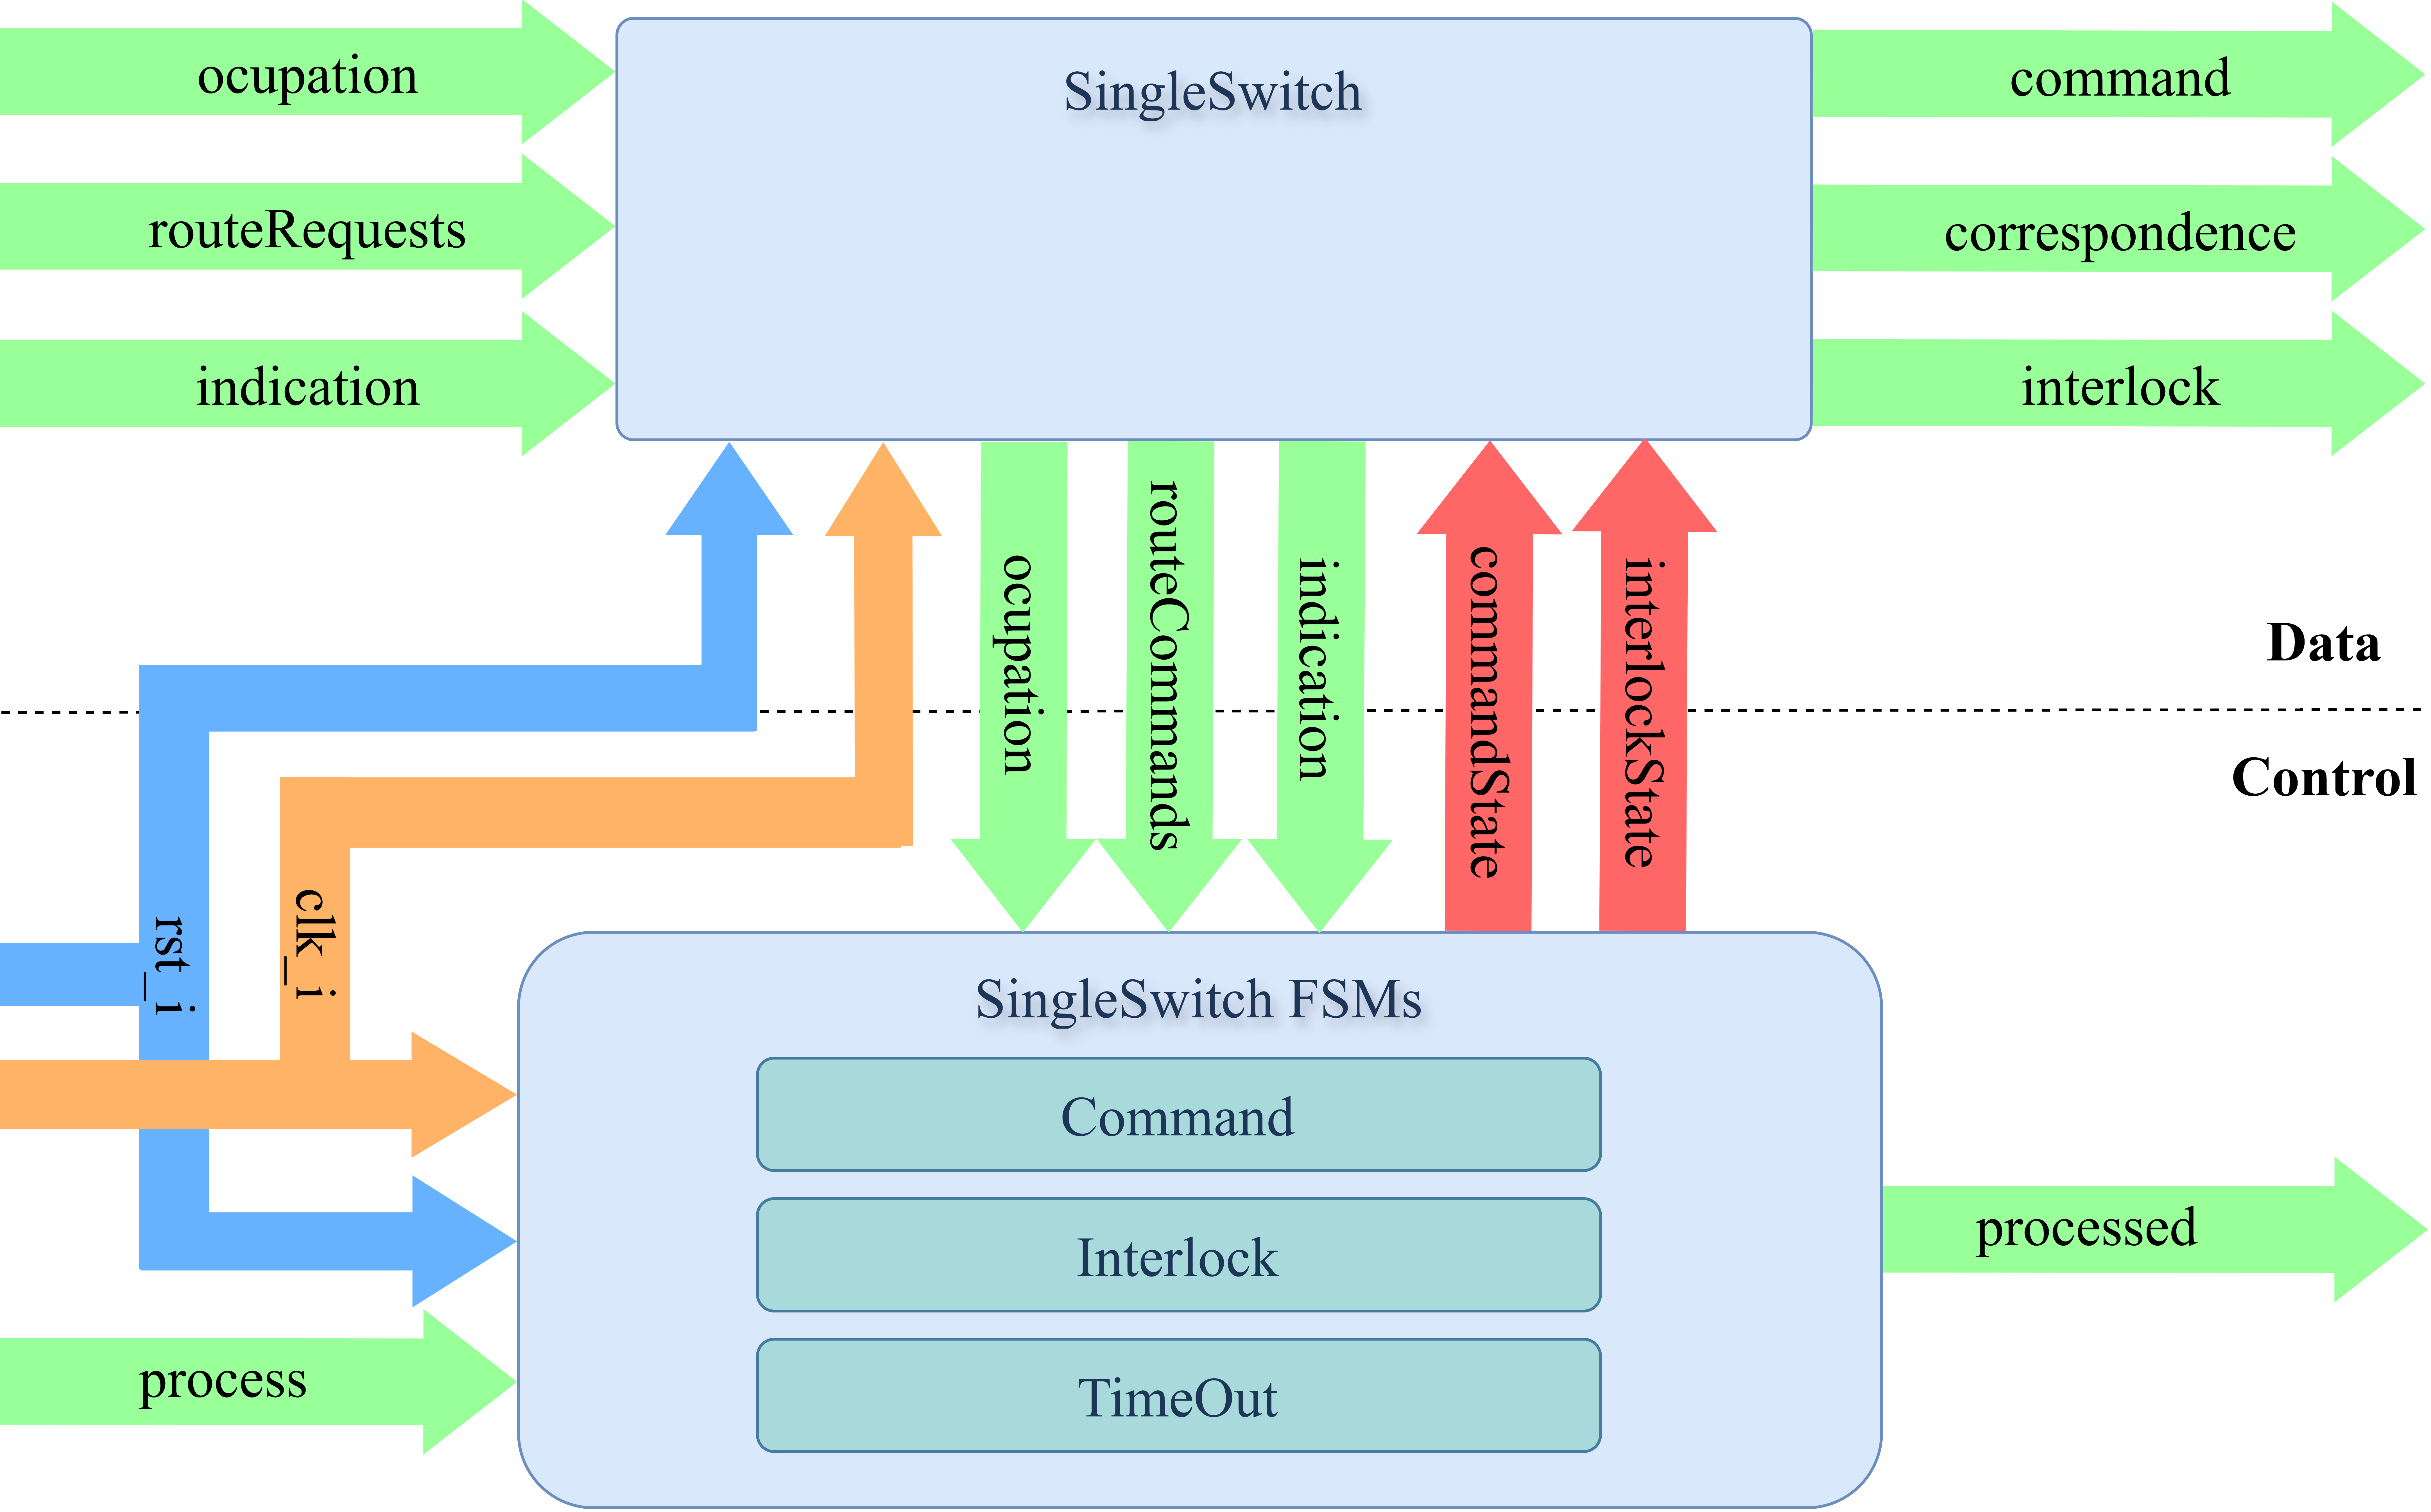
\includegraphics[width=1\textwidth]{Figuras/SSW_module}
		\centering\caption{FSMD del módulo genérico de \textit{SingleSwitches}.}
		\label{fig:SSW_module}
	\end{figure}
	
	Como fue explicado en la Sección \ref{sec:switches}, un cambio de vías simple puede adoptar dos posiciones: normal y reversa. Adicionalmente, es necesario contemplar que mientras la indicación no reporte una posición definida, normal o reverse, se deberá asumir que el cambio de vías se encuentra en transición de un estado al otro. Dicha transición debe ser corta, ya que de no completarse el movimiento puede ser tanto que el cambio de vías se encuentra atascado cómo que el comando o la indicación se encuentren desconectados del actuador. Esta funcionalidad, junto con el comportamiento del cambio de vías genérico se define en la red de Petri de la Figura \ref{fig:SSW_Petri}.
	
	\begin{figure}[H]
		\centering
		\includegraphics[width=1\textwidth]{Figuras/SSW_Petri}
		\centering\caption{Red de Petri del modelo dinámico de \textit{SingleSwitches}.}
		\label{fig:SSW_Petri}
	\end{figure}
	
	Un cambio de vías en estado reversa iniciará su transición si alguna de las rutas envía un comando para modificar la posición a normal, siempre que el cambio de vías no se encuentre enclavado por otra ruta que lo esté utilizando. Durante la transición, salvo que ocurra un timeout, el cambio de vías pasará al estado normal si se confirma la indicación normal y no el comando normal no fue cancelado por la ruta. Análogamente, el cambio de vías puede pasar del estado normal al reversa mediante la secuencia opuesta. Debiendo cumplir las mismas condiciones de no estar enclavado antes de mover el cambio de vías, confirmación de indicación y comando, y realizar todo el proceso dentro de un tiempo determinado.
	
	En el caso del timeout, se considera que si el cambio de vías no reporta una posición final en menos de un tiempo determinado, entonces el cambio de vías debe volver al estado anterior, de ser posible. De lograrse este o no, el cambio de vías igualmente quedará anulado y no podrá ser utilizado por la ruta que lo demanda, prohibiendo la habilitación de dicha ruta.

	\subsection{Módulo genérico de los cambios de vías dobles}

\lipsum[1]

\begin{figure}[H]
	\centering
	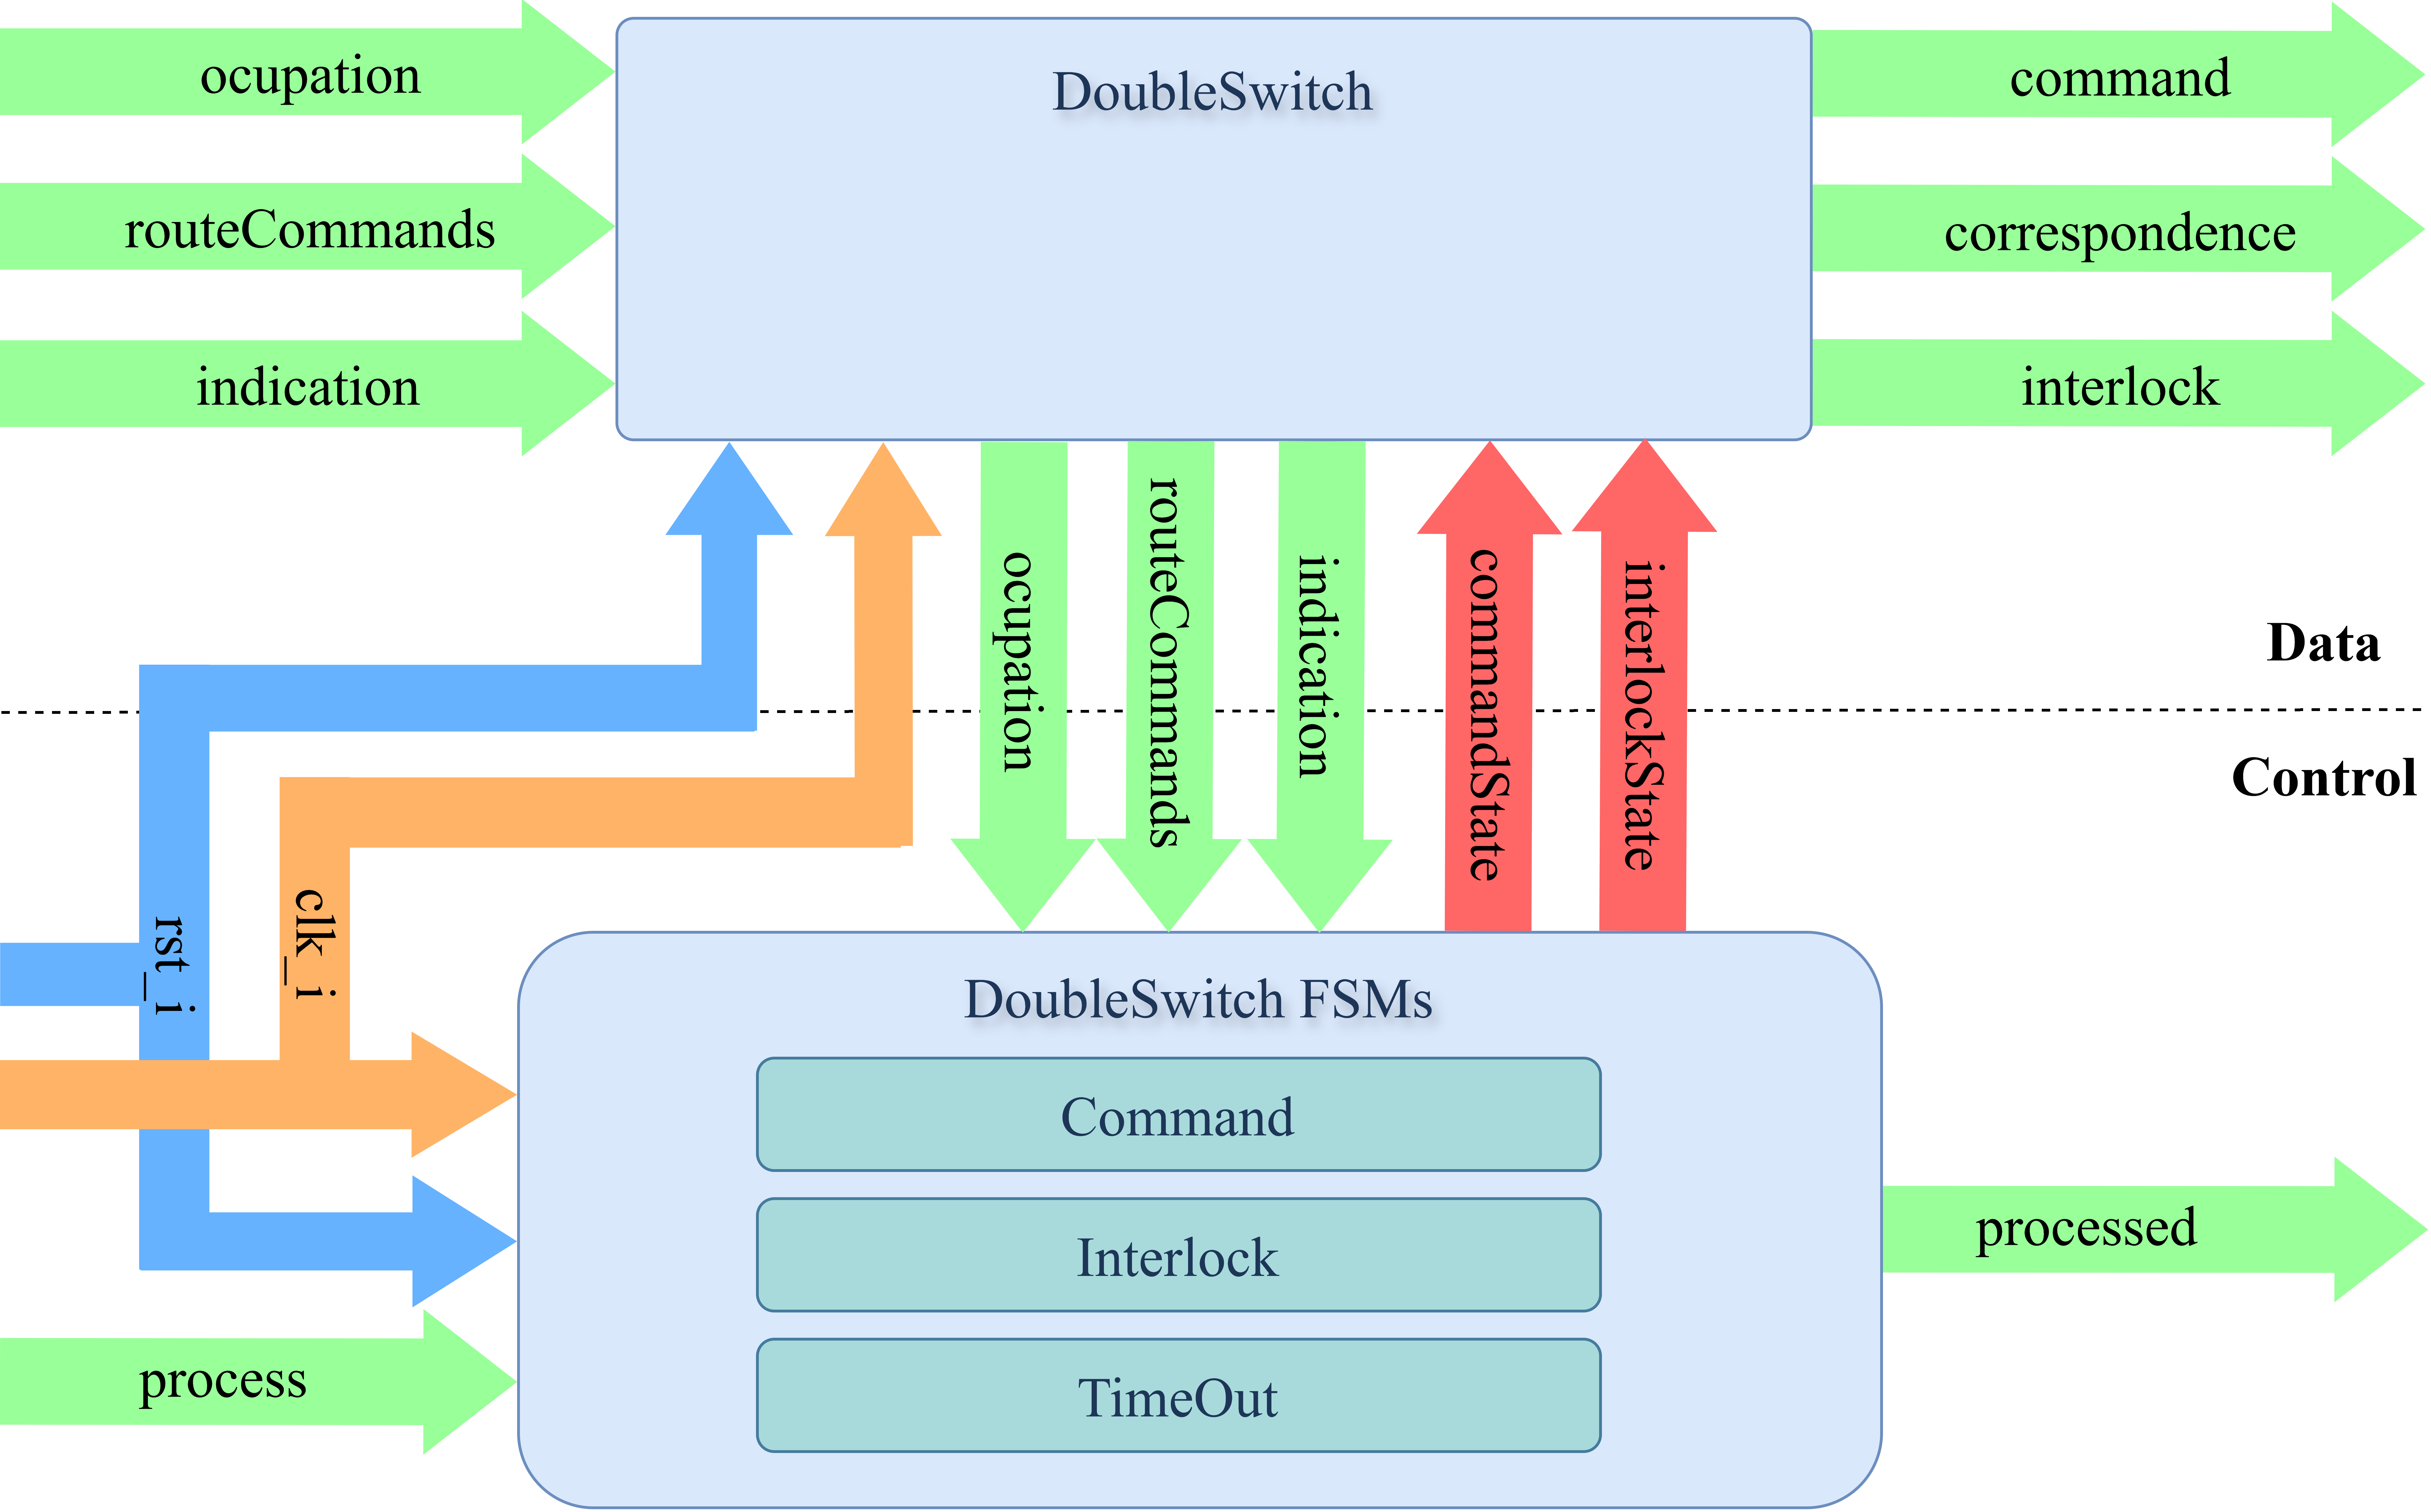
\includegraphics[width=1\textwidth]{Figuras/DSW_module}
	\centering\caption{FSMD del módulo genérico de \textit{DoubleSwitches}.}
	\label{fig:DSW_module}
\end{figure}

\lipsum[1]
	\subsection{Módulo genérico de los cambios en tijeras}

\lipsum[1]

\begin{figure}[H]
	\centering
	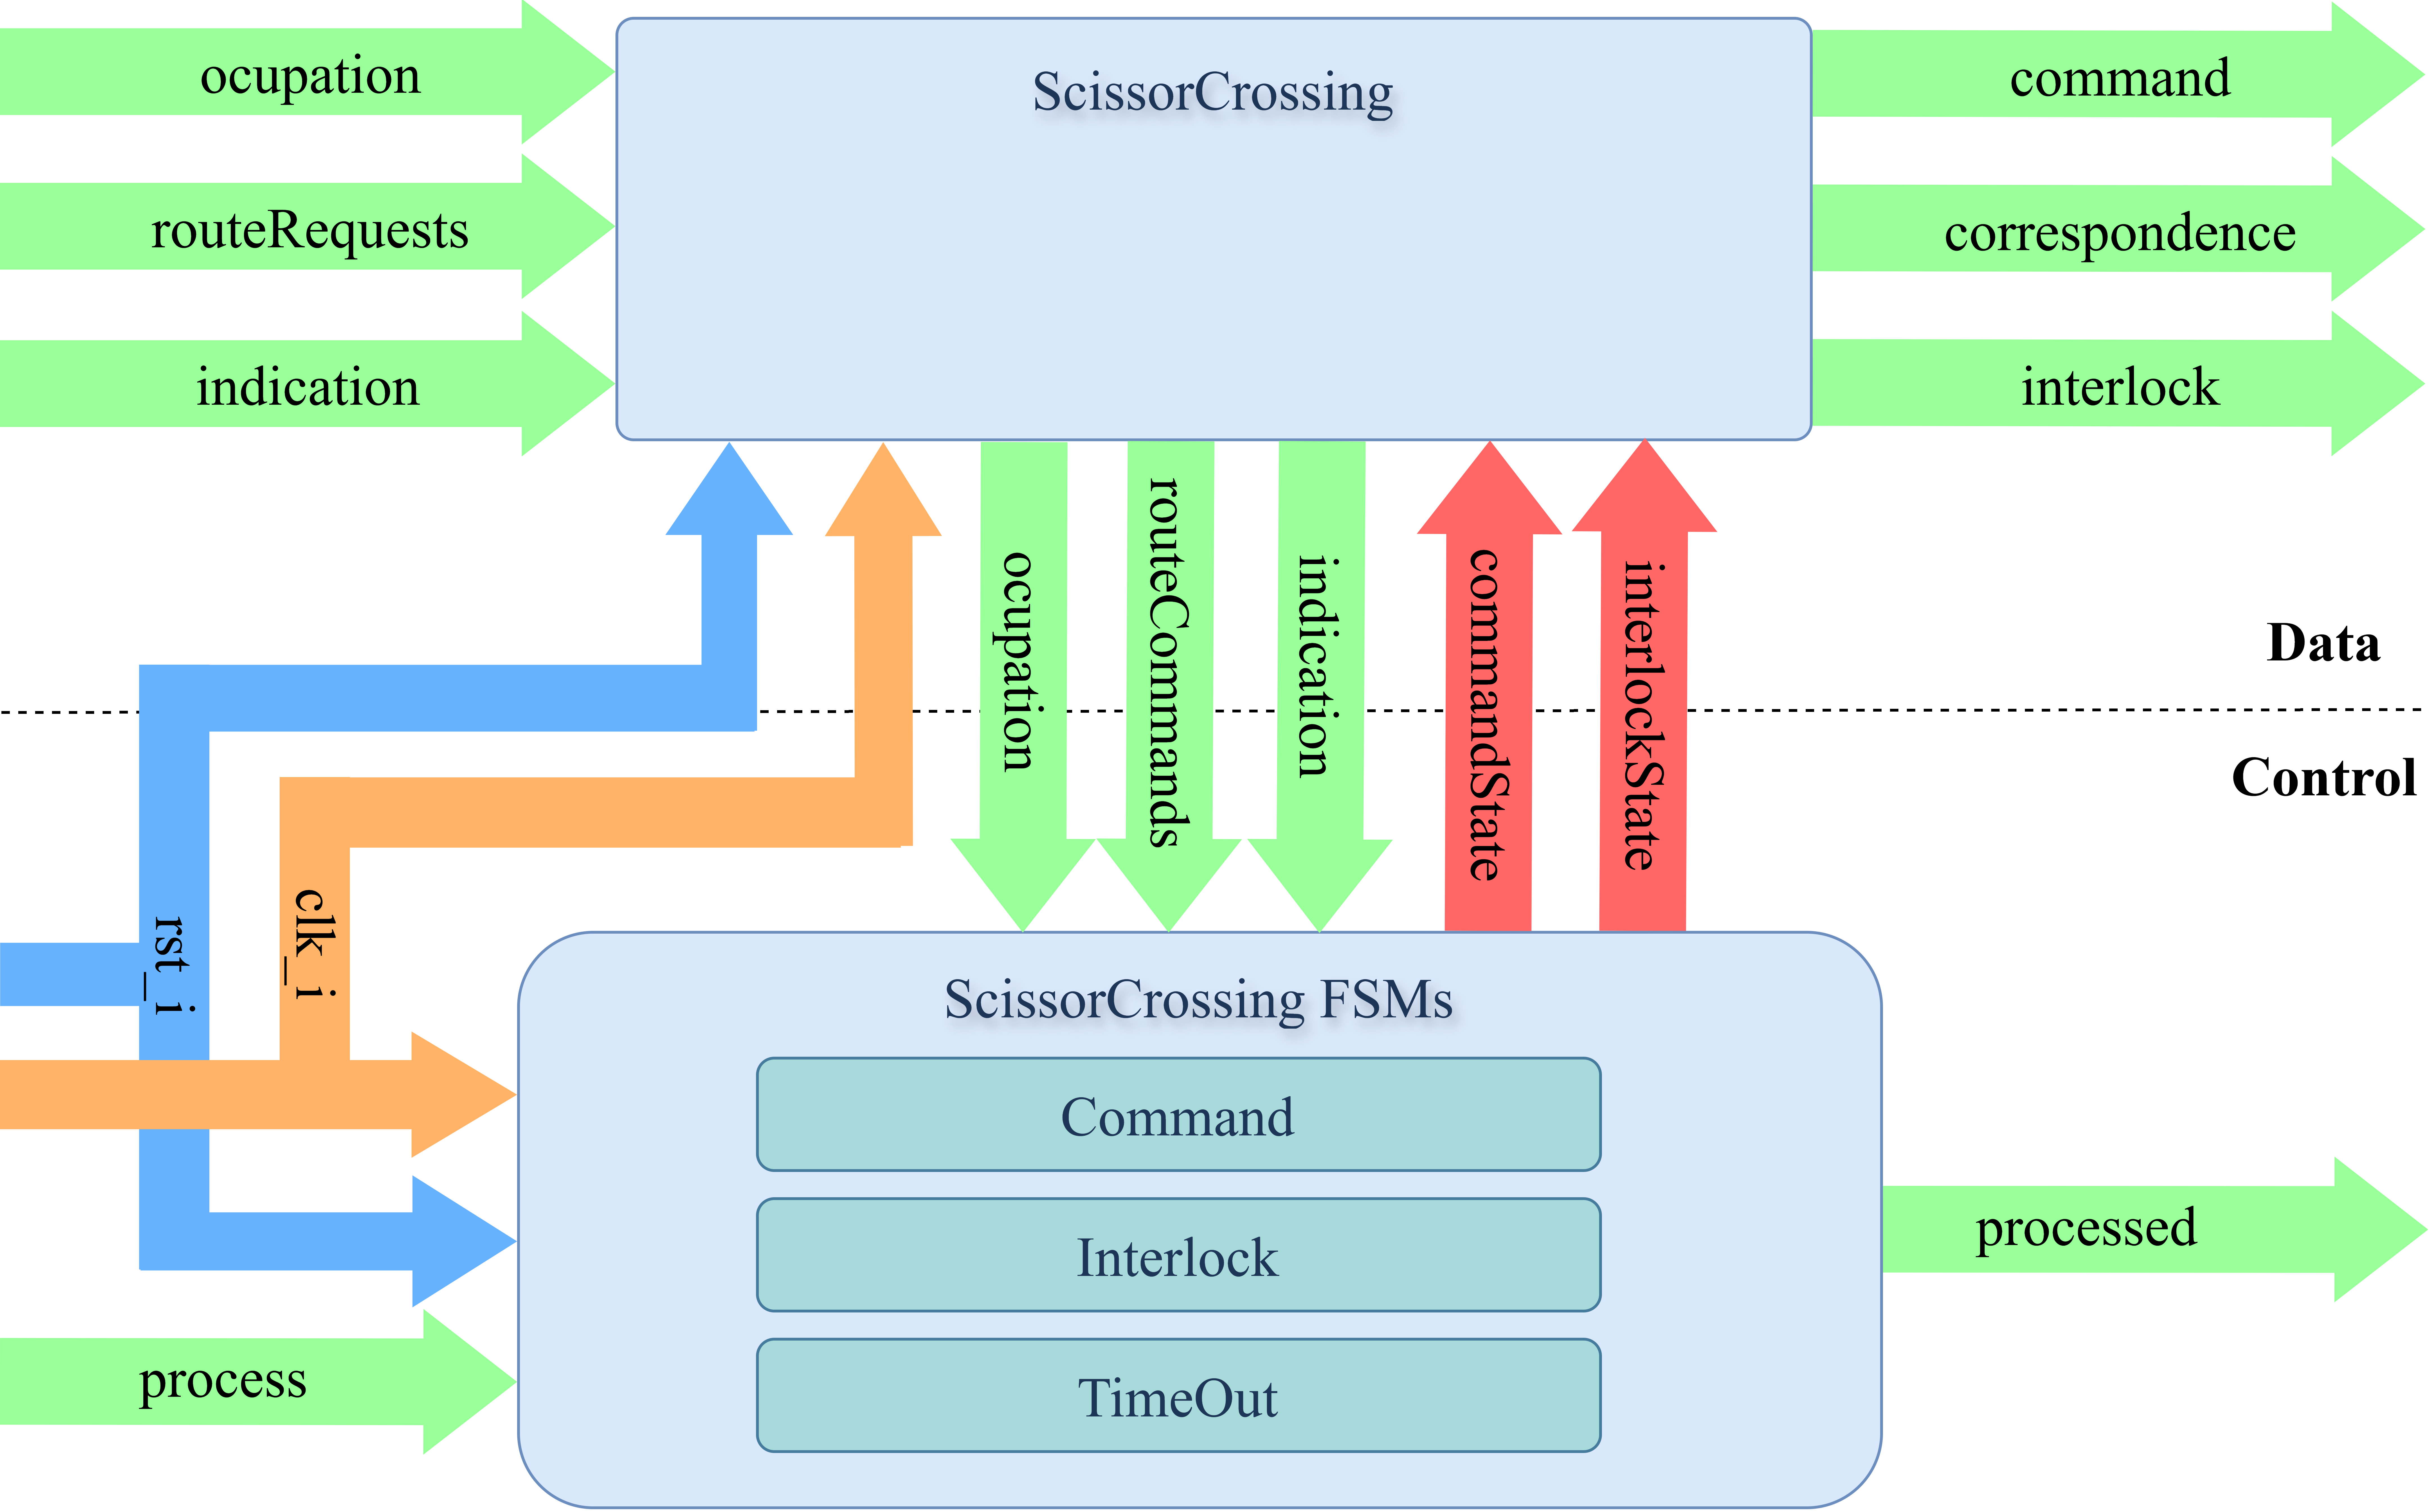
\includegraphics[width=1\textwidth]{Figuras/SCR_module}
	\centering\caption{FSMD del módulo genérico de \textit{ScissorCrossings}.}
	\label{fig:SCR_module}
\end{figure}

\lipsum[1]
	\subsection{Módulo genérico de los netElements}

El módulo \textit{NetElements} es el encargado de implementar el reporte del estado de ocupación de las vías. A diferencia de otros módulos centrados en el funcionamiento de mecanismos ferroviarios, leyendo su estado y enviando comandos para operarlo; el módulo de \textit{NetElements} solo se ocupa de reportar estados de sólo lectura, la presencia o no de una formación ferroviaria en una vía determinada, sin poder modificar sus valores de ninguna manera.

El ACG utiliza la información otorgada por el RNA para determinar las entradas y salidas cada módulo \textit{NetElements}, implementando uno por cada \textit{NetElement} definido en la red. Cada uno de estos módulos tendrá sus propios \textit{NetElements} leyendo su estado (\textit{ocupation}) y recibiendo consultas de las rutas que los solicitan (\textit{routeCommands}). A su vez, deberán a las rutas que los utilizan cuál es su estado (ocupado o libre, en el puerto \textit{state}) y si se encuentran enclavados (liberados, reservados o enclavados; en el puerto \textit{interlock}). El diagrama de bloques de las máquinas de estado finitas con camino de datos diseñado para lograr este objetivo se muestra en la Figura \ref{fig:NET_module}.

\begin{figure}[H]
	\centering
	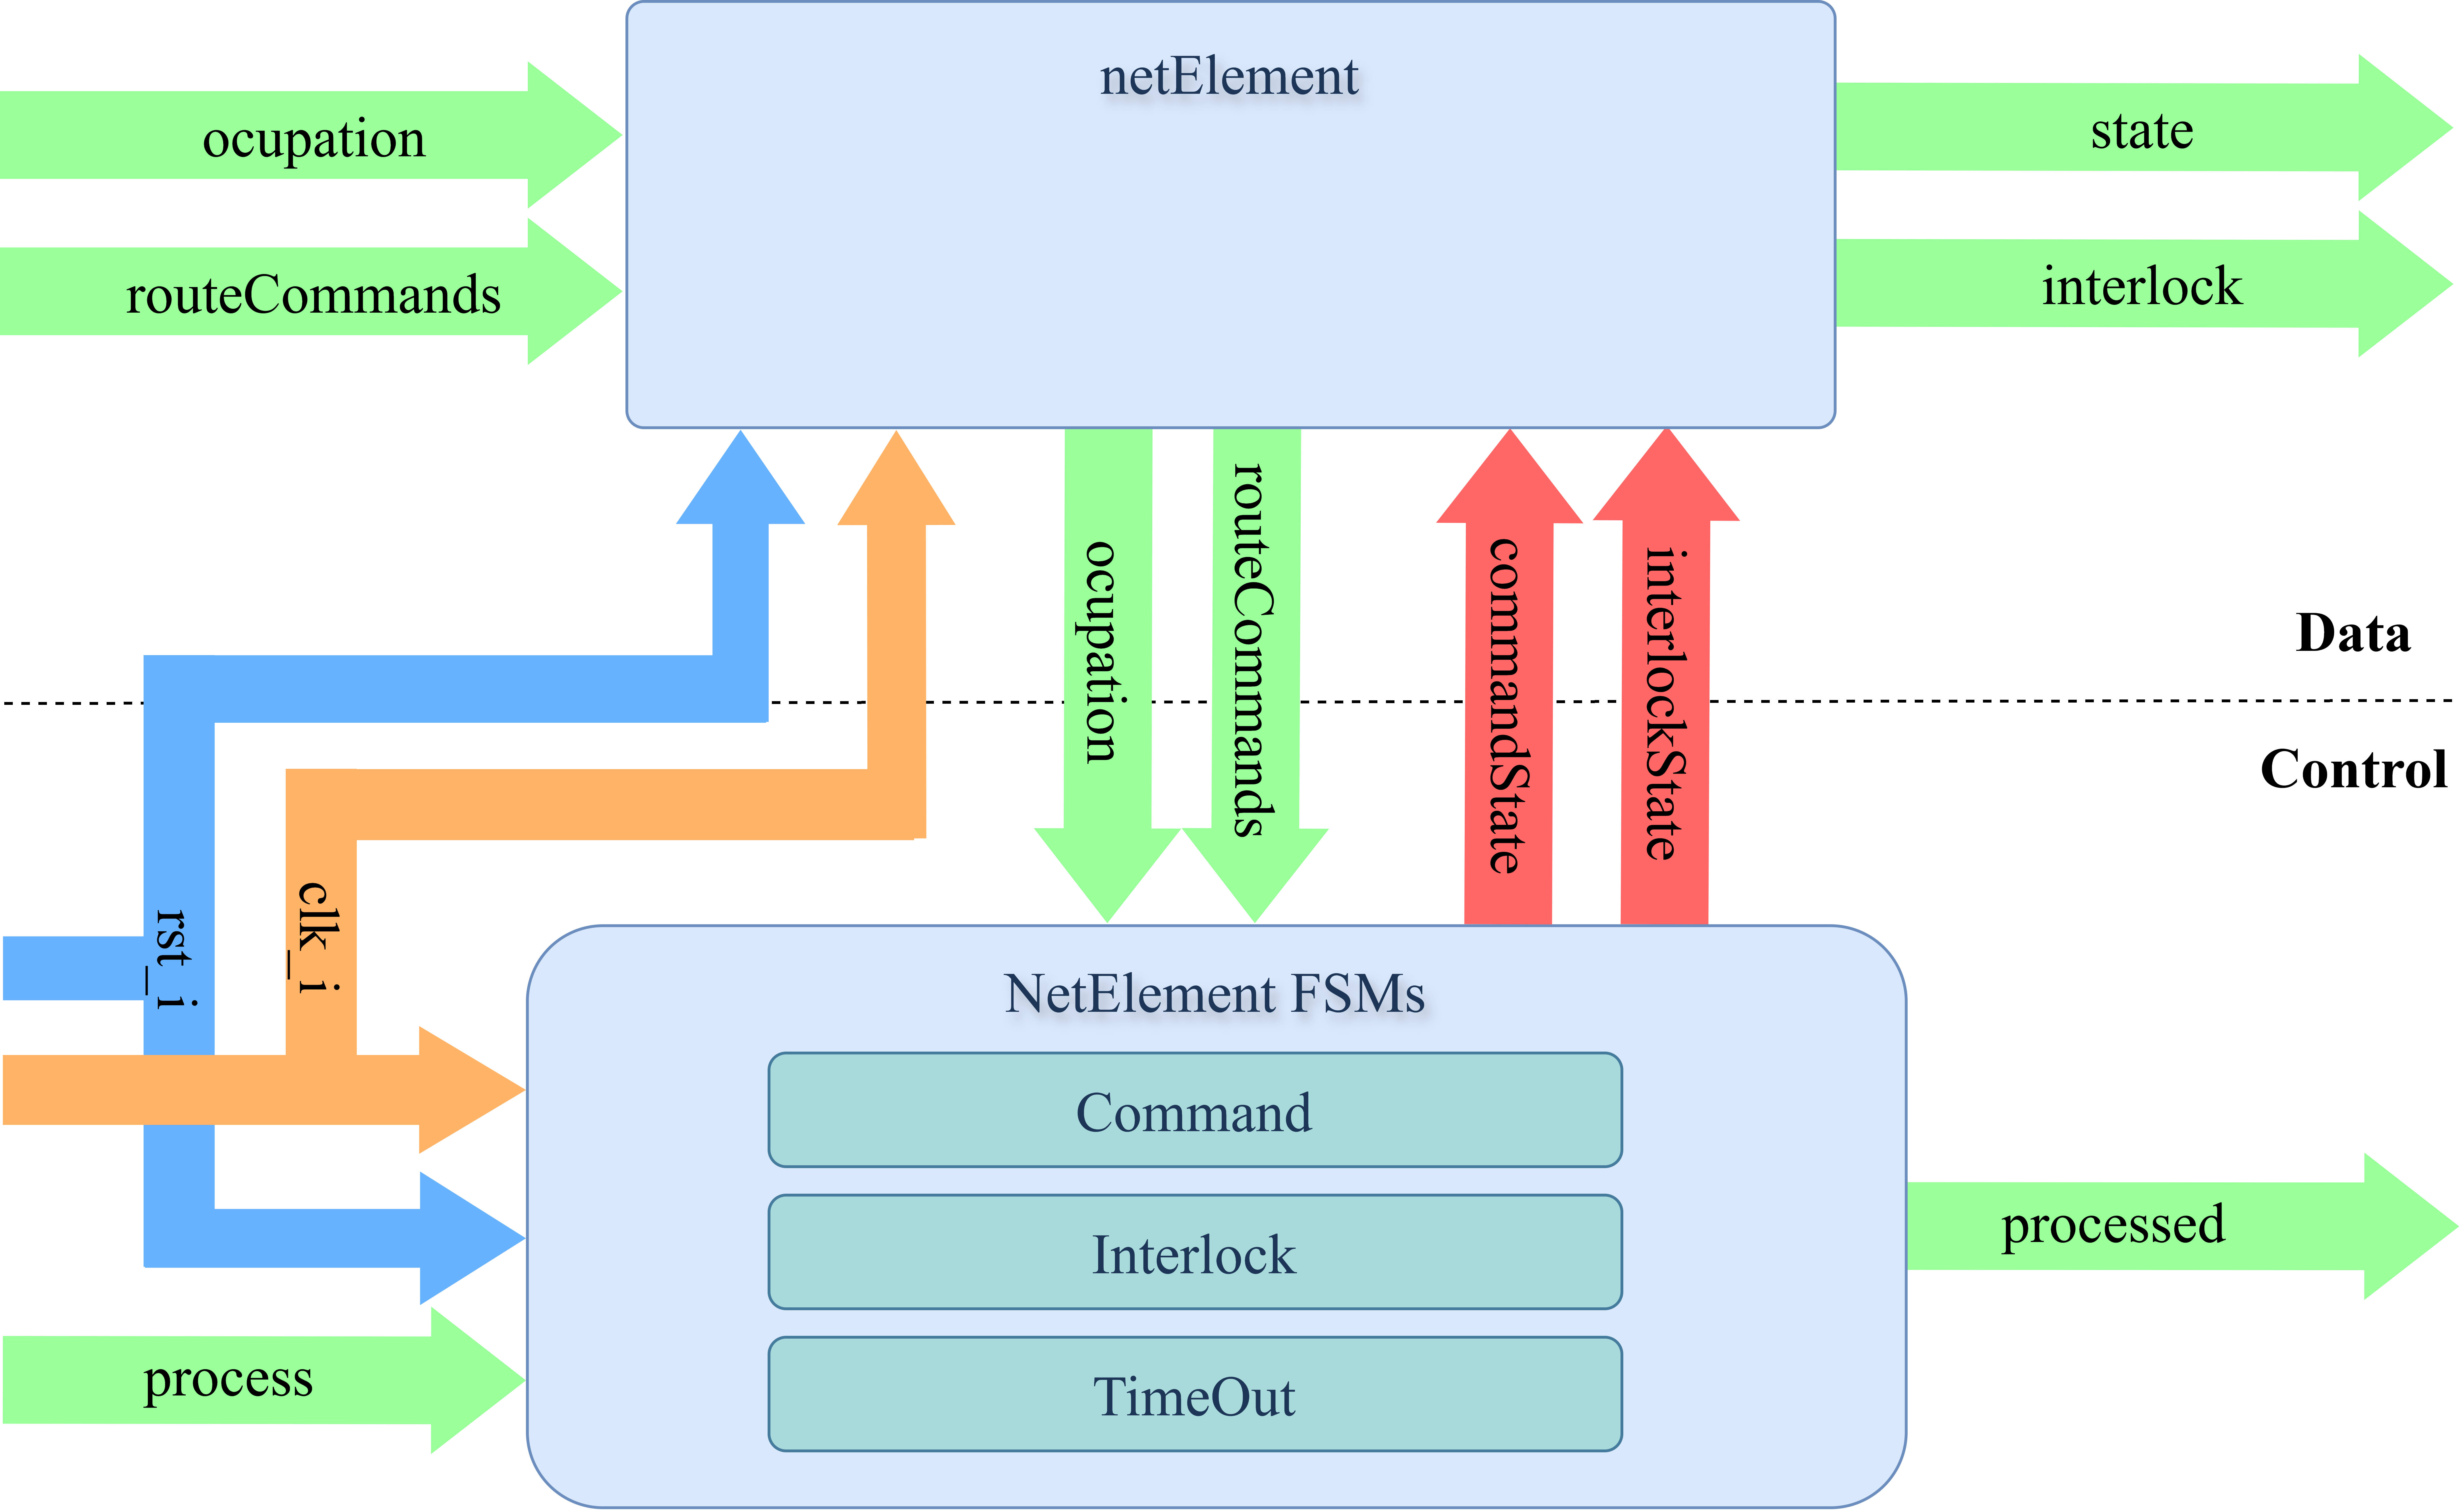
\includegraphics[width=1\textwidth]{Figuras/NET_module}
	\centering\caption{FSMD del módulo genérico de \textit{NetElements}.}
	\label{fig:NET_module}
\end{figure}

Cualquier ruta que pase por sobre el \textit{NetElement} en cuestión puede consultar su estado utilizando el puerto \textit{routeCommands}. Como ya fue explicado en la Sección \ref{sec:detectors}, un circuito de vía asociado a un \textit{netElement} puede estar ocupado por una formación o libre. Todos los módulos \textit{NetElements} reportaran su estado, independientemente si se encuentran reservados o enclavados. La reserva o enclavamiento es meramente para ser utilizado por las rutas para no considerar como propio un \textit{NetElement} que se encuentra libre pero ya ha sido reservado por otra ruta antagónica. El comportamiento del reporte del estado de ocupación de las vías se define en la red de Petri de la Figura \ref{fig:NET_Petri}.

\begin{figure}[H]
	\centering
	\includegraphics[width=0.75\textwidth]{Figuras/NET_Petri}
	\centering\caption{Red de Petri del modelo dinámico de \textit{NetElements}.}
	\label{fig:NET_Petri}
\end{figure}

La simpleza de la implementación del módulo \textit{NetElements} facilita una rápida respuesta por parte del sistema de enclavamientos, al otorgar la información requerida solamente a las rutas que la solicitan, reduciendo enormemente la cantidad de puertos y conexiones a implementar. El ACG creara, además, todas las conexiones necesarias entre cada módulo de elementos ferroviarios y los módulo \textit{NetElements} que los contienen, además de los vecinos mas próximos, para disminuir las chances de que ocurran situaciones peligrosas.
	\subsection{Módulo genérico de las señales ferroviarias}
	\label{sec:ACG_sig}
	
	El módulo \textit{Signals} es el encargado de implementar el funcionamiento de las señales ferroviarias. El ACG determine cuantos caminos posibles existen utilizando como punto de partida la señal ferroviaria a implementar. Cada uno de los caminos posibles influirá en el comportamiento de la señal ferroviaria. Para determinar cual es el único camino posible, el ACG implementa los puertos y conexiones a cada uno de los elementos ferroviarios involucrados con esa señal y hasta dos señales futuras, para todos sus caminos. En base a los estados reportados por estos elementos ferroviarios, el módulo \textit{Signals} determinará cuál es el camino activo y su señal ferroviaria quedará definida totalmente. El diagrama de bloques de las máquinas de estado finitas con camino de datos diseñado para lograr este objetivo se muestra en la Figura \ref{fig:SIG_module}.
	
	\begin{figure}[H]
		\centering
		\includegraphics[width=1\textwidth]{Figuras/SIG_module}
		\centering\caption{FSMD del módulo genérico de \textit{Signals}.}
		\label{fig:SIG_module}
	\end{figure}
	
	Como fue explicado en la Sección XXX, el aspecto de una señal ferroviaria será rojo si el conjunto de \textit{netElements} al que habilita circular la formación ferroviaria se encuentra ocupado. Si se encontrasen desocupados, su aspecto dependerá del aspecto de la señal siguiente. Pero cuál es la señal siguiente dependerá del estado actual de toda la infraestructura entre la señal analizada y dos señales consecutivas. El comportamiento del aspecto de una señal ferroviaria se define en la red de Petri de la Figura \ref{fig:SIG_Petri}.
	
	\begin{figure}[H]
		\centering
		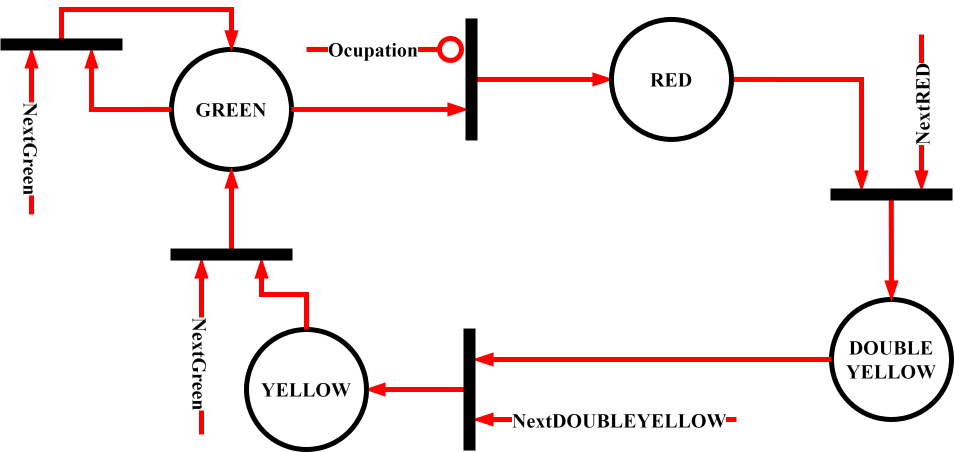
\includegraphics[width=1\textwidth]{Figuras/SIG_petri}
		\centering\caption{Red de Petri del modelo dinámico de \textit{Signals}.}
		\label{fig:SIG_Petri}
	\end{figure}
	
	La red de Petri ilustrada en la Figura \ref{fig:SIG_Petri} es una simplificación de la implementación real, solamente se ilustra un único cambio de estado entre un aspecto y otro. De haber ilustrado todas las transiciones entre, por ejemplo, el aspecto rojo y amarillo, el aspecto rojo y verde, o el aspecto rojo consigo mismo, entonces la cantidad de transiciones sería tres veces mayor.
	
	Teniendo en cuenta el modelo simplificado, una señal ferroviaria depende de si misma solo si la sección a la que protege se encuentra ocupada, en cuyo caso su aspecto será rojo. En caso contrario, si la sección se encuentra libre, dependerá del aspecto de la señal siguiente: si la señal siguiente es roja, el aspecto de la señal analizada será doble amarillo; si la señal siguiente es doble amarilla, el aspecto de la señal analizada será amarillo; si la señal siguiente es amarilla, el aspecto de la señal analizada será verde y, finalmente, si la señal siguiente es verde, el aspecto de la señal analizada también lo será.
	
	Las señales ferroviarias no pueden cambiar su aspecto una vez que se encuentran enclavadas, salvo para adoptar un aspecto mas restrictivo, para garantizar un mayor nivel de seguridad.
	\subsection{Módulo genérico de las rutas ferroviarias}

\lipsum[1]

\begin{figure}[H]
	\centering
	\includegraphics[width=1\textwidth]{Figuras/RTS_module}
	\centering\caption{FSMD del módulo genérico de \textit{Routes}}
	\label{fig:RTS_module}
\end{figure}

\lipsum[1]